\documentclass[a4paper,11pt]{article}

% With the commands after % signs you can define your own page size. Remove % to activate them and insert the values you want to define the size of the page you want.
    %\voffset=-2cm
    %\hoffset=-0.5cm
    %\textwidth=15cm
    %\parindent 0pt
    %\parskip 2ex
\setlength{\parindent}{24pt}
\setlength{\oddsidemargin}{-5mm}
\setlength{\evensidemargin}{-5mm}
\setlength{\textwidth}{165mm}
\setlength{\textheight}{230mm}
\setlength{\topmargin}{-10mm}
\setlength{\marginparwidth}{15mm}
\setlength{\marginparsep}{7mm}
%\setlength{\cftsecnumwidth}{2.3cm}


\usepackage{datetime}
\usepackage{graphicx,natbib}
\usepackage{gensymb}
\usepackage[colorinlistoftodos]{todonotes}
\usepackage{titling}
%provide smart links in your document
\usepackage{hyperref}

\newcommand{\subtitle}[1]{%
  \posttitle{%
    \par\end{center}
    \begin{center}\large#1\end{center}
    \vskip0.5em}%
}

% use double spacing for easy markup on the document for corrections
%\usepackage{setspace}
%\doublespacing

\newcommand{\tick}{\ding{51}}
\newcommand{\cross}{\ding{55}}

\newcommand\T{\rule{0pt}{3.5ex}}       % Top strut
\newcommand\B{\rule[-2.3ex]{0pt}{0pt}} % Bottom strut

\newdateformat{mydate}{%
    \monthname[\THEMONTH] \THEYEAR%
    }

\begin{document}
\bibliographystyle{spr-mp-sola}

% Front matter 
\title{End of First Year Report}
\subtitle{Draft}
\author{Georgina Long}

\date{\mydate\today}

\maketitle


\section{Introduction}

Ocean eddies are the subject of many ongoing investigations into ocean dynamics. The topic comprises a broad range of smaller-scale dynamics and relationships at varying scales. From energy transfer to blah blah *citations*, researchers are still trying to get a better understanding of the internal dynamics of the ocean. *citations*. Our main focus will be on the area of the Gulf Stream and mainly the interaction and effect of the bathymetry on the separation and subsequent path of the Gulf Stream.
\todo{Haven't added citations}

\subsection{The impact of an accurately resolved Gulf Stream}
\begin{itemize}
  \item Impact on other weather events - e.g.  \citep{Scaife2011a}
  \item Effect on other ocean processes and circulation - "blue spot of death"    %\todo{NW corner. Forntal path to west}
\end{itemize}
The Gulf Stream is part of the AMOC and is essential to transferring heat from the Gulf of Mexico at lower latitudes towards western and northern Europe. Fundamentally it gives north-western Europe its mild climate and thus has large impacts on the weather and climate as the heat is transferred into the atmosphere. This can have wide ranging effects on weather prediction – notably winter blocking \citep{Scaife2011a} and *other citation* \todo{I'm sure I read about cyclones somewhere - find citation}. Many lower resolution models render an unrealistic Gulf Stream, with the separation from the U.S. coast too far to the South, causing an inaccurate path from this point onwards. This obviously has a knock-on effect as the corresponding sea surface temperatures (SSTs) are much higher/lower than observed in the surrounding areas \citep{Greatbatch2004}\todo{check this is the right citation}. The cold bias in the North West corner of the Atlantic resulting from a poorly placed Gulf Stream has become known as the "blue spot of death" \citep{Gnanadesikan2007} to modellers due to the inaccuracies. The Northern Recirculation Gyre (NRG) interacts with the Gulf Stream and it has been noted by \citep{Zhang2007} and \citep{Ezer2016b}\todo{check this citation} that the representation of the Gulf Stream can have large effects on the energy modelled within the NRG \todo{\& the subtropical gyre too? – check this}. A lethargic NRG subsequently affects the *citations/TODO find out about this* and hence we can see that a poorly resolved Gulf Stream can have much wider implications throughout the model.

\subsection{Problems and Restrictions}
%\begin{itemize}
%  \item Many people restricted to coarser resolution models due to the cost of high resolution models but need high resolution to get a more accurate Gulf Stream - it's expensive to be accurate
%  \item We don't understand the smaller processes involved. \citep{Nikurashin2012a}
%\end{itemize}
Higher resolution models have been shown to provide a more realistic Gulf Stream path *citations*, however this comes at a cost requiring more processing power and thus a higher price for the model. It is generally understood *citations \citep{Nikurashin2012a} etc.* that this improvement is due to the higher resolution models being able to resolve small-scale processes which are lost in the coarser resolution counterparts. \citep{Ezer2016b} suggests that to replicate an accurate Gulf Stream separation, the model not only needed to resolve the Gulf stream but also the northern branches of NRG, the southward slope and shelf currents. \todo{Could the bathymetry cause an unresolved northern branches of NRG?}. *citation* It is also thought that the lack of detailed representation of the bathymetry in key areas play a large role in the unrealistic Gulf Stream path. *citation* posed that it is the interaction with the bathymetry and the consequential small-scale processes which cause the Gulf Stream to split off from the coast at Cape Hatteras and direct it’s path from there. The bathymetry itself can be represented in many different ways and the vertical coordinate system chosen has a large impact on the interaction of the ocean dynamics and the ocean floor. \citep{Ezer2016b} revisited a discussion on different vertical coordinate systems and their effect on the path of the Gulf Stream, though noted that the tested z-coordinate system did not include any partial or shaved cells. \todo{partial \& shaved cells - Mike's paper?}


\section{Background}
Tell a story up to where we are and what's missing.
\subsection{Literature Review (take most from coursework).Cover the various angles including:}
\begin{itemize}
  \item Modelling \& vertical grid systems - include partial cells
  \item Turbulence and bathymetry - understanding the smaller processes (vorticity etc.) \citep{Tansley2001} \citep{Nikurashin2012a}
  \item Possible relationships/data sets to see the history of the Gulf Stream. (Palaeo?) \citep{Ezer2015}
  \item Inclulde some phenomenology - e.g. bottom vortex stretching and bottom pressure torque. Maybe also the weird sandwhich diagram!
\end{itemize}

Cut down lit review - parts of it will be elsewhere!! (or should be! OR Remove them from elsewhere to keep them here!!)

\section{Lit Review as is.... Need to update it /TODO{update!!}}

\subsection{Introduction}
Ocean eddies are the subject of many ongoing investigations into ocean circulation. The topic comprises a broad range of dynamics and relationships at varying scales. By interpreting data and assessing the accuracy of models, scientists aim to gain a better understanding of the processes that govern the oceans.

Vast amounts of energy are contained within the ocean and it is still not fully understood how this energy is transported or dissipated into other processes \citep{Nikurashin2012a}. These processes which are still being questioned could provide insight into some of the areas that ocean models struggle to accurately represent.

One key area is the Gulf Stream, which despite being reasonably well represented in high resolution models, tends to be problematic in moderate and low resolution models \citep{Zhang2007}. This review aims to discuss the the various problems associated with modelling the Gulf Stream, with specific attention to the effect of bathymetry on its separation and subsequent path.


\subsection{Background}
The Gulf stream is part of the Atlantic Meridional Overturning Circulation (AMOC) and together with its extension, the North Atlantic Drift, carries warm water from the Gulf of Mexico, up the Florida coast, and then across to Western Europe. The resulting heat transported by the Gulf Stream contributes to the mild climate in Western Europe. Hence, understanding the Gulf Stream is important to obtain more accurate weather forecasts, as well as providing insight into the processes governing the dynamics themselves. It has been noticed that the Gulf Stream is slowing down and weakening over time \citep{Greatbatch1991}. This could have a significant impact on European weather, as an accurately resolved Gulf Stream in climate models has been linked to improved Atlantic winter blocking \citep{Scaife2011a}. \citep{Ezer2015} also investigated Atlantic circulation changes as a contributing factor to floods between Cape Hatteras and Cape Cod in the U.S., and sought a relationship between various currents and circulation in the North Atlantic with sea level changes on the Eastern coast of America. As observational data to determine the strength of the Gulf Stream has only been available for several decades, little is known about the evolution of the Gulf Stream over time. 

A good understanding of the Gulf Stream and it's contributing factors is crucial for improved climate and ocean models. The misrepresentation can not only lead to inaccurate but also false data. The warm and cold biases in sea surface temperatures (SSTs) throw off climate predictions and could be obscuring climate change predictions \citep{Saba2016}.


\subsubsection{Gulf Stream Separation}

The Gulf stream separates at Cape Hatteras, skirts the Grand Banks at Newfoundland and then heads Eastwards towards western Europe. However, in many moderate resolution climate models this separation occurs further north than observed and turns more sharply to the East, as noted in \citep{Hurlburt2008} and often misses off the Grand Banks, heading straight towards Europe. This can lead to what modellers refer to as the "blue spot of death" \citep{Gnanadesikan2007}, a patch of colder than observed SSTs resulting from the lack of heat at Newfoundland normally brought up by the Gulf Stream.

The exact cause for the path of the Gulf Stream is unknown, though it has been a research topic for many years and is still a popular topic amongst researchers today. A recurring theme when looking into the separation of the Gulf Stream is the mention of bathymetry. It is thought \citep{Gula2014}\citep{NaveiraGarabato2013}\citep{Nikurashin2012a} that the ocean dynamics resulting from the interaction of the Gulf Stream and the deep western boundary current (DWBC) with the bathymetry in the North Atlantic could cause the turbulence required to direct the Gulf Stream along its path. A sudden change in the direction of the Gulf Stream just off the coast at South Carolina and Georgia has been attributed to the Charleston Bump, a topographical feature which raises the ocean floor, from a depth of 600m on the surrounding Blake Plateua to 200m \citep{Gula2014}. Hence it is clear that bathymetry can strongly impact the direction of ocean currents.


\subsubsection{Small-scale Processes}

It has been noted that in higher resolution models, the separation and subsequent path of the Gulf Stream is much more accurate than in the lower resolution counterparts \citep{Hurlburt2008}\citep{Zhang2007}. This lends to the idea that the processes which affect the Gulf Stream occur on smaller scales which aren't resolved by coarser models \citep{NaveiraGarabato2013}\citep{Nikurashin2012a}. Various processes have been investigated and suggested as the main influences though it is likely that the improved Gulf Stream representation is due to multiple factors.


\citep{NaveiraGarabato2013} theorised that interaction with the bathymetry creates small-scale turbulence and instabilities which could cause bathymetric steering and divert currents. If this is not being represented in coarser models, the energy behind the turbulence must be going elsewhere. \citep{Scott2010} compared current meter readings with modelled values for kinetic energy and noticed that in some areas of the North Atlantic the total kinetic energy was being held higher in models than observed. It is discrepancies such as this which could have much wider implications. If the energy is not penetrating to the ocean floor, we cannot expect to be able to replicate the effects of the bathymetry. Perhaps by pulling this energy further down (closer to observed values), there would be more energy transfer from the larger ocean eddies to the smaller scale turbulence resulting from interaction with the bathymetry.

\citep{Tansley2001} used a simplified model of water flowing past a cylinder to highlight the importance of turbulence on fluid motion. Using a quarter-cylinder ( mimicking a simplified version of Cape Hatteras) and a high Reynolds number (allowing for more turbulent flow), the model produced a jet with surrounding turbulent eddies similar to those observed in the Gulf Stream. These results were not seen with a lower Reynolds number, highlighting the importance of turbulence in forming jets like the Gulf Stream.

The turbulent mixing arising from interaction with the bathymetry could allow geostrophic eddies to transfer some of their energy to smaller processes by causing internal waves to break and contribute to enhanced mixing \citep{Nikurashin2012a}. These effects have been seen even in cases of small-scale bathymetric roughness suggesting that it is not necessary to have large topological features to impact ocean dynamics, instead small surface differences can cause changes which lead to bigger outcomes.

\citep{NaveiraGarabato2013} attribute the significant impact of small-scale bathymetry to wave drag. Although wave drag is not a large contributor to ocean dynamics, topological features on a small scales can cause wave drag which contributes ten to several tens of a percentage of the dominant source and sink terms influencing the vorticity of the ocean.


These effects of small-scale processes are not limited to the Gulf Stream, but impact on many aspects of ocean dynamics as the various currents and features affect one another. 
\citep{Ezer2016} speculated that amongst other things, the northern branches of the Northern Recirculation Gyre (NRG) would have to be resolved in order to produce an accurate Gulf Stream in a model. \citep{Zhang2007} determined that a significant contribution to the generation of the NRG is the bottom vortex stretching resulting from a downslope DWBC, which is in turn the result of the interaction with bathymetry as the DWBC crosses the path of the Gulf Stream. Hence, bathymetric impact can circle around to affect many aspects of ocean dynamics.


\subsubsection{Modelling the Gulf Stream}

As more scientists seek to understand ocean dynamics, more models are made and used by different researchers to simulate different processes. There are many models in use today, all with different configurations and settings. This can lead to contrasting outcomes and debate over which choice of model or model settings yields the most accurate results.

%\subsubsubsection{Model Resolution}/TODO subsubsubsection
\paragraph{Model Resolution}

\subparagraph
	Along with differing numerical schemes or boundary conditions, etc. there are also many different model resolutions available. These range from coarse 1$\degree$ models, which resolve to a scale of $\approx$ 100km, to higher resolution 0.25$\degree$ models, which resolve to a scale of $\approx$ 25km, all with varying numbers of vertical levels. It is well established \citep{Scaife2011a}\citep{Hurlburt2008} that a higher resolution ocean model tends to produce a more accurately resolved Gulf Stream. This is in part due to the small scale processes, mentioned previously, which contribute to the ocean circulation, but are not resolved in the coarser models. Unfortunately higher resolution models require additional processing power and thus additional costs. This means that the high resolutions required to resolve a realistic Gulf Stream will not be widely used for some time. Hence, the aim is to find a way to represent an accurate Gulf Stream in the lower resolution models by understanding the reasons behind it.

%\subsubsubsection{Vertical Coordinate System} /TODO subsubsubsection
\paragraph{Vertical Coordinate System}

\subparagraph
	One of the main variabilities between different models is the handling of the vertical coordinate system. The way in which the model splits the depth of the ocean into 'levels' can have a large impact on the way the bathymetry is represented. As previously discussed, this bathymetric representation can have large impacts on the dynamics within the model. The importance and significance of the bathymetric roughness has already been discussed in this review so it is now necessary to discuss the different ways to represent this.
\subparagraph
The main coordinate systems in use are the z-coordinate system which stays true to a cartesian system of coordinates, consisting of rectangular 'blocks', which create a staircase effect when representing slopes. These z-coordinate systems can also be implemented with 'partial cells' whereby some of the cells are cut into smaller cells to 'smooth out' and more closely represent the shape of the slopes. Thre are also s- (or sigma-) coordinates which follow the shape of the terrain. The depth at any point is divided by the number of levels to create a consistent number of cells at all points of different thickness. These different approaches can also be combined to form hybrid coordinate systems. See Figure \ref{fig:coords} for an illustration of some of the possible vertical coordinate systems available in the NEMO model.

\begin{figure}
  \centering
  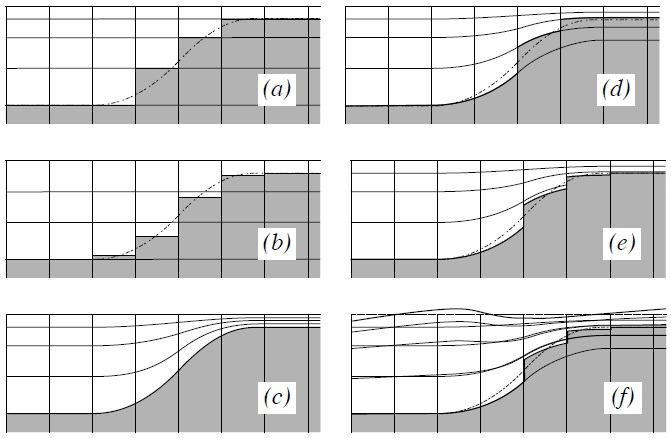
\includegraphics[scale=.8]{NEMOP58.jpg}
  \caption{An illustration of different veritcal coordinate systems available in NEMO. \citep{Madec2011}. (a) z-coordinate, (b) z-coordinate with partial cells, (c) s-coordinate, (d) hybrid s-z coordinate, (e) hybrid s-z coordinate with partial cell, (f) shows (e) with a non-linear free surface (which can be used with any coordinate system).}
  \label{fig:coords}
\end{figure}

\subparagraph
The main difficulty in comparing different vertical coordinate systems lies in the availability of a 'control' case for the comparison. With the wide selection of models available to researchers, it is not only the vertical coordinate system which differs but also the numerical schemes being used to resolve various processes. This could lead to false similarities or differences and cause incorrect conclusions. \citep{Ezer2016} was able to compare results from z-coordinate models and s-coordinate models while minimalising any other differnces between the models. Although the z-coordinate models are capable of producing an accurate Gulf Stream at hight resolutions, the s-coordinate models provided a more accurate representation when restricted with coarser models. However, as \citep{Ezer2016} noted in the comparison, partial and shaved cells (whereby corners of the cells are 'shaved' off to smooth out slopes) were not used in any of these models.


\subsection{Discussion}

After evaluating the progress made so far and the themes that researchers are focusing, there are a few areas which invite further exploration.

There is scope for further investigation into vertical coordinate systems. Building on the work of \citep{Ezer2016}, including partial cells and hybrid coordinate schemes on model comparisons could provide interesting results of the Gulf Stream representation across different model resolutions. As the improved results in higher resolution models has highlighted the importance of small-scale processes, these kind of investigations could lead to further insight into understanding ocean dynamics.

The evolution of the Gulf Stream and it's changes in direction and strength over time \citep{Greatbatch1991} tells an interesting story and could itself shed light on contributing factors. For example links drawn between different currents could lead to understanding of the impact they have on each other as \citep{Ezer2015} suggested that Gulf Stream changes could be impacting the slope current rather than the other way around as previously suspected.

Many of the theories of smaller-scale processes come with proposed parametrisations (whether specifically included with the research or posed as future work), see \citep{NaveiraGarabato2013} amongst others, and there are other schemes proposed for more general processes such as the one proposed by \citep{Anstey2016} for mesoscale eddies which fell outside the scope for this review. As researchers, we should be aiming towards a parametrisation scheme which could allow the effects of rough bathymetry (and the resulting sub-scale processes) to be taken into account without the need of a higher resolution to resolve the bathymetry itself (thus reducing the necessity and thus costs for high resolution models). However, a deeper understanding of the causes and effects involved would be required than is currently obtained.

\subsection{Conclusion}

We have discussed the ideas and challenges facing researchers when trying to understand and improve the model of the Gulf Stream. A combination of physical processes, their causes and ultimate representation in ocean models holds the key to accurately reproducing the separation and path of the Gulf Stream. This topic continues to inspire lots of research into the areas of ocean eddies, bathymetric interaction and model configurations, as more accurate simulations and higher levels of understanding lie in the future




\section{Results}

Results so far - link into Background \& lead nicely into the next section.
\subsection{Barotropic vorticity diagnostics}
\begin{itemize}
  \item Results so far
  \item Discussion on results and possible implications
  \item Results on what we're looking at and why
  \item Maybe brief description of JEBAR etc. to explain it's use \& who else has used it to show what - e.g. why are we looking at it etc?
  \item Should probably include model set up
\end{itemize}



\section{Future Aims/Questions}

We seek a robust \& accurate Gulf Stream path. How can we improve the representation \& thus understanding of the Gulf Stream?

We seek to improve the understanding and representation of the Gulf Stream in moderate resolution models. As we have discussed, there are many processes involved in the dynamics of the ocean and thus there are many different directions to turn to when seeking solutions to this problem. Here we will focus on the interactions and effects of the bathymetry while being careful not to ignore other paths this investigation may lead down. 

\subsection{Identifying key processes}
\begin{itemize}
  \item Understanding
  \item Representation
\end{itemize}

It is speculated *paper*\todo{female author?} that interaction with the bathymetry creates small-scale turbulence and instabilities which can cause bathymetric steering and divert currents. If this is not being represented in coarser models, the energy behind the turbulence must be going elsewhere. \todo{paper}*paper* compared simulated kinetic energy over different models against measurements taken and noted that in some areas the total kinetic energy was being held higher in the ocean in the models than observed. It is discrepancies \todo{choose a different word} such as this which could have much wider implications. If the energy is not penetrating to the ocean floor, we cannot expect to be able to replicate the effects of the bathymetry. Perhaps pulling this energy further down (closer to observed values), we would be able to see the energy transfer from \todo{?}*** to the turbulence resulting from the bathymetry. 

Of course as previously discussed there are many processes which could contribute to a Gulf Stream path staying too far South. \citep{Ezer2016b} speculated that amongst other things, the northern branches of the NRG would have to be resolved in order to produce an accurate Gulf Stream. \citep{Zhang2007} determined that a significant contribution to the generation of the NRG is the bottom vortex stretching resulting from a downslope DWBC, which is in turn the result of the interaction with the bathymetry as the DWBC crosses the path of the Gulf Stream. Thus we see that this circles back to interaction with the bathymetry.


\subsection{Different model formulations}
\begin{itemize}
  \item Representation of the bathymetry
  \item Effects of different vertical grids
\end{itemize}

The many different ocean and OGCM models available allow us to see the effects of many different schemes and parameterisations in use today. In particular the choice of vertical coordinate system has long been discussed, especially in regard to its relevance here. Obviously the representation of the topography and the way it is rendered in the model is a result of the vertical coordinate choice. \citep{Ezer2016b} revisited the discussion in relation to the Gulf Stream separation and used similar models to determine the most accurate results over different choices for coordinate systems. However, the z-coordinate system chosen did not include any partial or shaved cells. It is inherently obvious that using the z-coordinate system would cause the various slopes in the ocean floor to appear as ‘steps’ which would significantly alter the flow around the area. \todo{A diagram of the different coordinate systems?}. It is not so surprising perhaps that under these circumstances \citep{Ezer2016b} found sigma or s-coordinates to be the most realistic given that they allow for a smooth ocean floor. It is perhaps natural then to question the effect of partial or shaved cells on these findings. As NEMO allows for such a diverse range of configurations and schemes, it would be interesting to recreate these results while implementing a z-coordinate system with partial cells to allow for a new take on this review. \todo{Maybe move to the next section instead?}

\subsection{Gulf Stream interaction with other systems}
\begin{itemize}
  \item Interaction with other currents   (DWBC, etc.)
  \item Relationship with data sets
  \item Evolution of the Gulf Stream
\end{itemize}



\section{Lines of Enquiry \& Methodology}

\subsection{NEMO}
\begin{itemize}
  \item Model Resolution \citep{Ezer2016b}
  \begin{itemize}
    \item simple configurations? \citep{Tansley2001}
  \end{itemize}
  \item Representation of Bathymetry
  \begin{itemize}
    \item Vertical Coordinate Systems
    \item Partial Cells
    \item Nested grids (enhancing resolution in specific areas?) 
  \end{itemize}
\end{itemize}

To examine the aforementioned interplay between the NRG and the path of the Gulf Stream, a simple configuration of NEMO simulating the double gyre set-up seen by the NRG north of the Gulf Stream and the subropical(?) gyre south of the gulf stream could be used to examine the effects in an idealised model. Results from this could help to influence our investigations within the more realistic models. As \citep{Tansley2001} used the classic problem of flow past a cylinder to understand the Gulf Stream separation, we too can learn from idealised set up and by breaking the problem down to its fundamental aspects.

\subsection{Understanding the Gulf Stream}
\begin{itemize}
  \item Turbulence    (\&Geostrophic turbulence)
  \item Vorticity and it's contributors
\end{itemize}
  
It has been discussed previously \todo{here? Or do I need to recite?} that a lack of energy transfer, either by lack of interaction with the bathymetry, or via some other process, could be to blame for the low levels of turbulence found in the area surrounding the separation of the Gulf Stream. As seen when \citep{Tansley2001} used a larger Reynolds number, allowing for more turbulent flow, flow passing a quarter-cylinder (akin to the coastline at Cape Hatteras), formed jet like streams with smaller eddies breaking away  from it. This is akin to satellite observations of the Gulf Stream \todo{could I put a side by side of the two pictures here? Satellite v Tansley/Marshall picture?}. This leads to the question which many try to answer – how can we improve/enhance the turbulence in a model?   
  
\subsection{Gulf Stream Relationships}
\begin{itemize}
  \item Data Sets    \citep{Ezer2015}
  \begin{itemize}
    \item Explore the possible links between the Gulf Stream and other data sets (e.g. coastal sea level)
  \end{itemize}
  \item Impact of other currents    \citep{Ezer2015}
  \item Changes in the Gulf Stream \citep{Greatbatch1991} \citep{Ezer2015}
\end{itemize}


\section*{Notes}
\begin{itemize}
	\item Make lit review more specific - focus it on a few key papers rather than covering a ton of them!
	\item Focus on phenomenology rather than model stuff
	\item Add a section somewhere to explain bottom pressure torque and bottom vortex stretching - maybe in diagnostics secion but elsewhere too
	\item Maybe add in weird sandwhich scales phenomenology?
	\item Explain vertically integrated blah blah
	\item Find out a use for the vertical average info.
	\item Maybe discuss Sverdrup vs barotropic streamfunction transport? (see P2075 bottom right blue highlighted in Vallis \& Zhang 2007)
	\item Include how the energy is dissipated and where it goes when it hits the bottom - I think this was John T's q from my talk
	\item PHENOMENOLOGY
	\item What am I doing with the average?
\end{itemize}

%\bibliography{EoFYR}
\bibliography{../../../../bibtex/EoFYR}

%\newpage
%
%\appendix
%
%\part*{Appendices}
%
%
%\begin{thebibliography}{99}
%\bibitem{peccei}
%
%\bibitem{feynmandiag}
%
%\end{thebibliography}

\end{document}
